% Technical documentation of the proportional per-node damping package.
% Compile from the package root with:  xelatex DOCUMENTATION_EN.tex  (three times, for the table of contents)
\documentclass[11pt,a4paper]{article}
\usepackage[a4paper,top=2.5cm,bottom=2.5cm,left=2.2cm,right=2.2cm]{geometry}
\usepackage{amsmath,amsthm}
\usepackage{mathptmx}
\usepackage{amssymb}
\usepackage[no-math]{fontspec}
\usepackage[english]{babel}
\babelfont{rm}[Language=Default,RawFeature={-ccmp}]{FreeSerif}
\babelfont{sf}[Language=Default,RawFeature={-ccmp}]{FreeSans}
\babelfont{tt}[Language=Default,Scale=0.86]{DejaVu Sans Mono}
\usepackage{microtype}
\usepackage{booktabs}
\usepackage{array}
\usepackage{longtable}
\usepackage[font=small,labelfont=bf,skip=4pt]{caption}
\usepackage{enumitem}
\setlist{itemsep=2pt,topsep=3pt}
\usepackage{tikz}
\usetikzlibrary{arrows.meta,positioning}
\usepackage{xurl}
\usepackage{xr-hyper}
\externaldocument[P-]{paper/paper_en}  % numbers of the paper's tables, figures and sections (compile the paper first)
\usepackage[hidelinks]{hyperref}
\usepackage{placeins}
\emergencystretch=2em

\newtheorem{theorem}{Theorem}
\newtheorem{lemma}{Lemma}
\newtheorem{corollary}{Corollary}
\theoremstyle{definition}
\newtheorem{remark}{Remark}
\theoremstyle{plain}
\newcommand{\genpropname}{}
\newtheorem*{genprop}{\genpropname}
\newenvironment{prop}[1]{\renewcommand{\genpropname}{Proposition #1}\begin{genprop}}{\end{genprop}}

\newcommand{\Pesc}{P_{\mathrm{esc}}}
\newcommand{\Pescbar}{\bar{P}_{\mathrm{esc}}}
\newcommand{\clip}{\mathrm{clip}}
\newcommand{\diag}{\mathrm{diag}}
\newcommand{\E}{\mathbb{E}}
\newcommand{\N}{\mathcal{N}}
\newcommand{\AP}{\mathrm{AP}}
\newcommand{\one}{\mathbf{1}}
\newcommand{\file}[1]{\path{#1}}

\input{paper/generated/macros.tex}
\input{paper/generated/tables_en.tex}

\title{\textbf{Self-Consistent Proportional Per-Node Damping for Reachability Ranking in Uncertain Graphs}\\[4pt]
\large Technical documentation: architecture, proofs, code walkthrough, complexity and reproduction guide}
\author{Ioannis Konstantellos\\[2pt]
\small Computer Engineering and Informatics Department\\
\small University of Patras, Greece}
\date{October 2026}

\begin{document}
\maketitle

\begin{abstract}
\noindent This document accompanies the paper \emph{Self-Consistent Proportional Per-Node Damping for Reachability Ranking in Uncertain Graphs: Exact Theory, Dynamical Obstructions, and Hybrid Dual-Operator Polishing} and its Greek version. It describes the architecture of the software package that produced every number in the paper, gives complete proofs of Theorem~1 and of Propositions~A--F and~$2'$ together with the auxiliary lemmas on which the implementation relies, walks through every module, analyses the time and memory complexity of each component, and gives a step-by-step guide for reproducing the experiments, the tables, the figures and the four PDF documents from scratch.
\end{abstract}

\tableofcontents

\section{Scope and conventions}\label{sec:scope}

The package studies the Proportional Relative Influence Principle for per-vertex damping in diffusion-based reachability ranking. It contains (i)~a vectorised library implementing uncertain-graph instances, Monte Carlo ground truth, propagation operators, damped diffusions, message passing, the three realizations of the principle, the anchored power family, Mode~(b) polishing, oracles and metrics; (ii)~the experiment runners for a pre-registered evaluation on \NTotal{} instances; (iii)~analysis, control and benchmarking scripts; and (iv)~the generators of every macro, table and figure of the paper.

Notation follows the paper. $G=(V,E,p)$ is an undirected uncertain graph with $n=|V|$ vertices and $m=|E|$ edges, each present independently with probability $p_{ij}\in(0,1]$; $x>0$ with $\sum_ix_i=1$ is the prior; $y^*_i=\E\big[\sum_{v\in C(i)}x_v\big]$ is the expected reachable mass. Vectors are compared componentwise, $\circ$ is the componentwise product, $\N(v)=v/\one^{\top}v$ and $\one$ is the all-ones vector. In file names, \file{<panel>} is one of \texttt{dev}, \texttt{test}, \texttt{prior}, \texttt{real}, \texttt{scale}. In result files a step count $T=10^6$ stands for ``run to the fixed point'' ($T=\infty$).

\section{Architecture}\label{sec:architecture}

\subsection{Repository layout}

Table~\ref{tab:layout} lists the files and directories of the package.

\begin{longtable}{>{\raggedright\arraybackslash}p{5.3cm}>{\raggedright\arraybackslash}p{10.3cm}}
\caption{Repository layout.}\label{tab:layout}\\
\toprule
Path & Content \\
\midrule
\endfirsthead
\caption[]{Repository layout (continued).}\\
\toprule
Path & Content \\
\midrule
\endhead
\file{prop_damping_lib.py} & The library: instances, priors, real-network loading, operators, Monte Carlo and exact ground truth, metrics, diffusions, message passing, the realizations, the anchored law, polishing, oracles. \\
\file{build_panels.py} & Generates the five panels and their two independent ground-truth samples. \\
\file{experiments.py} & The \texttt{grid} stage (full search on dev and test) and the \texttt{confirm} stage (references, oracles and the frozen configurations on the held-out panels). \\
\file{select_configs.py} & Re-derives the frozen configurations from the development results by the stated rules and verifies \file{results/selected.json}. \\
\file{analysis.py} & Loading of stage results, configuration means, paired statistics, Holm correction. \\
\file{controls.py}, \file{mf_controls.py} & Matched controls: constant damping, per-step mean (mean-field twin) and permutation of the per-node law. \\
\file{sign_condition.py}, \file{prop2_stats.py} & Diagnostics for Proposition~E (sign condition) and Proposition~2 (prior uniformity). \\
\file{explore_rawP.py} & Exploratory (not pre-registered) raw-$P$ propagation. \\
\file{mc_baseline.py}, \file{bench_runtime.py} & Monte Carlo baselines at $k\in\{50,200,1000\}$ worlds and single-process timings. \\
\file{paper_extras.py} & Dynamics traces, operator complementarity and the size sweep. \\
\file{make_checkpoint_tables.py}, \file{write_checkpoint_report.py} & The tables and report of the first checkpoint. \\
\file{make_paper_assets.py}, \file{paper_figures.py} & Every macro, table and figure of the paper (English and Greek). \\
\file{tests/} & Foundational and dynamical checks (Theorem~1, ground truth, propositions). \\
\file{data/<panel>/NNNN.npz} & Instances with their ground truth; \file{data/<panel>/specs.json} lists the specifications. \\
\file{results/} & Per-instance results, controls, diagnostics, timings, the frozen selection and its digest. \\
\file{paper/} & \file{paper_en.tex}, \file{paper_gr.tex}, the generated assets in \file{paper/generated/} and the compiled PDFs. \\
\file{figures/}, \file{figures_gr/} & The five figures with English and Greek labels. \\
\file{logs/} & Progress logs of the long stages (used for the run times reported here). \\
\bottomrule
\end{longtable}

\subsection{Data flow}

Figure~\ref{fig:pipeline} shows the pipeline. Each stage reads only the outputs of earlier stages, so any stage can be rerun in isolation. Selection uses the development panel only, and every held-out stage reads the frozen configuration file.

\begin{figure}[!ht]
\centering
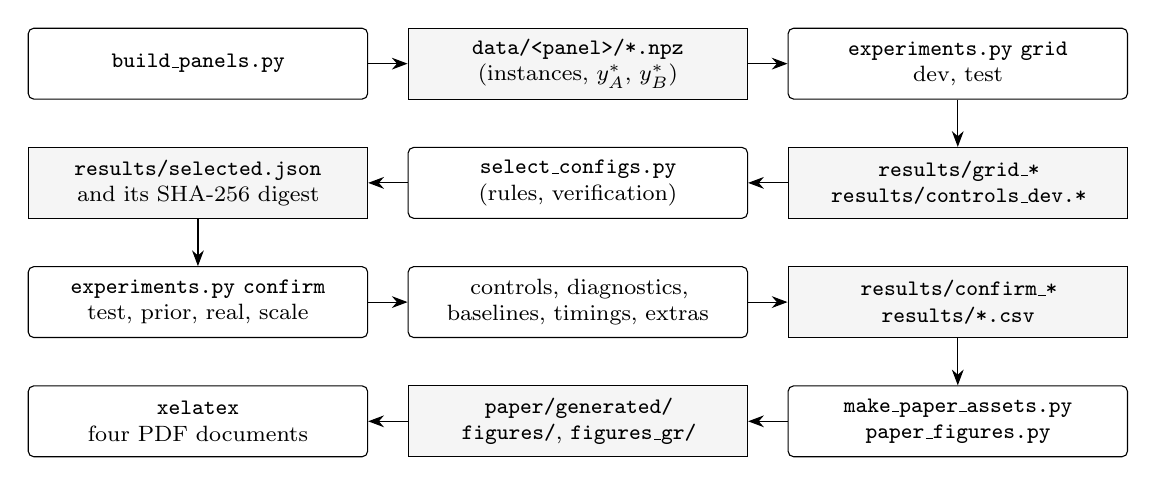
\begin{tikzpicture}[node distance=6mm and 5mm, font=\footnotesize,
  box/.style={draw, rounded corners=2pt, align=center, inner sep=3pt, minimum height=9mm, text width=4.1cm},
  data/.style={draw, align=center, inner sep=3pt, minimum height=9mm, text width=4.1cm, fill=black!4},
  arr/.style={-{Stealth[length=2mm]}}]
\node[box] (build) {\texttt{build\_panels.py}};
\node[data, right=of build] (data) {\texttt{data/<panel>/*.npz}\\(instances, $y^*_A$, $y^*_B$)};
\node[box, right=of data] (grid) {\texttt{experiments.py grid}\\dev, test};
\node[data, below=of grid] (gres) {\texttt{results/grid\_*}\\\texttt{results/controls\_dev.*}};
\node[box, left=of gres] (sel) {\texttt{select\_configs.py}\\(rules, verification)};
\node[data, left=of sel] (frozen) {\texttt{results/selected.json}\\and its SHA-256 digest};
\node[box, below=of frozen] (conf) {\texttt{experiments.py confirm}\\test, prior, real, scale};
\node[box, right=of conf] (aux) {controls, diagnostics,\\baselines, timings, extras};
\node[data, right=of aux] (res) {\texttt{results/confirm\_*}\\\texttt{results/*.csv}};
\node[box, below=of res] (assets) {\texttt{make\_paper\_assets.py}\\\texttt{paper\_figures.py}};
\node[data, left=of assets] (gen) {\texttt{paper/generated/}\\\texttt{figures/}, \texttt{figures\_gr/}};
\node[box, left=of gen] (tex) {\texttt{xelatex}\\four PDF documents};
\draw[arr] (build) -- (data);
\draw[arr] (data) -- (grid);
\draw[arr] (grid) -- (gres);
\draw[arr] (gres) -- (sel);
\draw[arr] (sel) -- (frozen);
\draw[arr] (frozen) -- (conf);
\draw[arr] (conf) -- (aux);
\draw[arr] (aux) -- (res);
\draw[arr] (res) -- (assets);
\draw[arr] (assets) -- (gen);
\draw[arr] (gen) -- (tex);
\end{tikzpicture}
\caption{Data flow of the package. Grey boxes are files; white boxes are programs.}
\label{fig:pipeline}
\end{figure}

\subsection{Determinism}

Every random draw is seeded by \texttt{stable\_seed(*parts)}, the first 63 bits of the SHA-256 digest of the role of the draw (for instance the panel, family, size, probability range and replicate of an instance, or the instance name and the purpose of a Monte Carlo sample). Seeds therefore do not depend on the order of execution or on the number of worker processes, and rerunning any stage reproduces the stored results bit for bit on the same platform. Topology and edge probabilities of a synthetic instance are seeded independently of its prior, which is what allows the prior panel to vary only the prior.

\subsection{File formats}

\paragraph{Instances.} \file{data/<panel>/NNNN.npz} stores \texttt{edges} (an $m\times2$ integer array with $i<j$), \texttt{p} (edge probabilities), \texttt{x} (prior), \texttt{yA} and \texttt{yB} (two independent \MGT-world ground-truth estimates), \texttt{yA2} (the second moment of the evaluation sample) and \texttt{meta} (a JSON string with family, size, probability range, prior, replicate, $\Pescbar$, prior statistics and the split-sample reference). \texttt{load\_instance} returns the instance, \texttt{yA}, \texttt{yB} and the metadata.

\paragraph{Results.} Each stage writes \file{results/<stage>_<panel>/<id>.csv.gz} with one row per evaluated method or configuration and the columns \texttt{id}, \texttt{method}, \texttt{T} (steps or sweeps; 0 for single-shot methods), \texttt{beta} (blend weight), \texttt{blend} (\texttt{s} score blend, \texttt{r} rank blend, \texttt{-} none) and \texttt{rho} (Spearman against $y^*_A$), plus a JSON file with diagnostics (oracle fits, dynamics, secondary metrics).

\paragraph{Method names.} The prefix of a method name identifies its family; the fields after the colon are separated by vertical bars.
\begin{center}\small
\begin{tabular}{>{\raggedright\arraybackslash}p{6.0cm}>{\raggedright\arraybackslash}p{9.4cm}}
\toprule
Prefix or pattern & Meaning \\
\midrule
\texttt{base:} & reference diffusions: \texttt{rule\_EW}, \texttt{fixed085}, \texttt{rule\_WT}, \texttt{local\_pesc} \\
\texttt{ref:} & references: \texttt{prior}, \texttt{Pesc}, \texttt{MP2}, \texttt{MPinf}, \texttt{ceiling} \\
\texttt{oracle:} & oracles: \texttt{scalar}, \texttt{scalar\_in}, \texttt{scalar\_WT}, \texttt{pernode} \\
\texttt{true:} & the per-node laws evaluated with the true $y^*$: \texttt{prop}, \texttt{ap0.5}, \texttt{ap1.0} \\
\texttt{sa:kind|op|scale|gamma} & standalone realizations \\
\texttt{ap:eta} & the anchored law \\
\texttt{free:gamma|eta} & the unanchored law \\
\texttt{pb:base|eta|mode} & anchored polishing (\texttt{fix}: fixed $\alpha$; \texttt{sc}: self-consistent) \\
\texttt{pbx:base|kind|op|scale|gamma} & realization polishing \\
\texttt{pbperm:base} & permuted anchored polishing \\
\texttt{sel:NAME} & a frozen configuration \\
\bottomrule
\end{tabular}
\end{center}

\paragraph{Frozen configurations.} \file{results/selected.json} maps each of the \NFrozen{} names to its parameters (Table~\ref{tab:configs}); \file{results/selected.sha256} records its digest (beginning with \texttt{\SelHash}) and the time it was frozen (\SelTime).

\TabConfigs

\section{Mathematical foundations}\label{sec:math}

This section collects every mathematical statement used by the paper or by the implementation, with complete proofs. Throughout, $T\ge0$ entrywise; $T$ is \emph{row-substochastic} if $T\one\le\one$; $\rho(\cdot)$ denotes the spectral radius.

\subsection{Auxiliary results used by the implementation}

\begin{lemma}[normalised damped diffusion]\label{lem:diffusion}
Let $\alpha\in[0,1]^n$, $D=\diag(\alpha)$ and $B(\alpha)=(I-D)\,x\,\one^{\top}+DT$. A vector $y>0$ with $\one^{\top}y=1$ is a fixed point of $y\mapsto\N\big((1-\alpha)\circ x+\alpha\circ Ty\big)$ if and only if it is an eigenvector of $B(\alpha)$ with eigenvalue $\lambda=\one^{\top}B(\alpha)y>0$; it then satisfies $\lambda y=(I-D)x+DTy$. If $\alpha_i<1$ for every $i$, then $B(\alpha)>0$ entrywise, the eigenvector is unique (the Perron vector), and both the plain and the lazy power iterations converge to it from every positive start. If $B(\alpha)$ is only irreducible (for instance $\alpha\equiv1$ and $T$ irreducible but periodic), the lazy iteration $y\leftarrow\N\big(\tfrac12(y+B(\alpha)y)\big)$ still converges to the Perron vector.
\end{lemma}

\begin{proof}
For $\one^{\top}y=1$ we have $B(\alpha)y=(I-D)x+DTy$, so the fixed-point equation $y=\N(B(\alpha)y)$ is $B(\alpha)y=(\one^{\top}B(\alpha)y)\,y$. If every $\alpha_i<1$, the rank-one term $(I-D)x\one^{\top}$ is entrywise positive, so $B(\alpha)>0$ and Perron's theorem~\cite{hornjohnson13} gives a simple, strictly dominant eigenvalue with a positive eigenvector, the only positive eigenvector up to scaling; the power method converges to it from every positive start. The lazy matrix $\tfrac12(I+B)$ has the same eigenvectors and eigenvalues $\tfrac12(1+\mu)$. If $B$ is irreducible with Perron root $r$, every other eigenvalue satisfies $|\tfrac12(1+\mu)|\le\tfrac12(1+|\mu|)\le\tfrac12(1+r)$, with equality only when $\mu=r$; hence $\tfrac12(1+r)$ is strictly dominant, and the lazy power method converges even when $B$ has other eigenvalues of modulus $r$ (periodic case).
\end{proof}

\begin{lemma}[anchoring constant]\label{lem:anchor}
For real numbers $\ell_1,\dots,\ell_n$ and $\alpha_0\in(0,1)$ there is a unique $c\in\mathbb R$ with $\frac1n\sum_i\sigma(c+\ell_i)=\alpha_0$, where $\sigma$ is the logistic function. A Newton iteration safeguarded by the bracket $[\mathrm{logit}(\alpha_{\min})-\max|\ell|-1,\ \mathrm{logit}(\alpha_{\max})+\max|\ell|+1]$ and by bisection converges to it.
\end{lemma}

\begin{proof}
$h(c)=\frac1n\sum_i\sigma(c+\ell_i)$ is continuous and strictly increasing, with $h(c)\to0$ as $c\to-\infty$ and $h(c)\to1$ as $c\to\infty$, so $h(c)=\alpha_0$ has exactly one solution, and it lies in the bracket because $h$ at the endpoints is below $\alpha_{\min}\le\alpha_0$ and above $\alpha_{\max}\ge\alpha_0$. The implementation keeps the bracket updated by the sign of $h(c)-\alpha_0$ and replaces any Newton step that leaves it by the midpoint, so the bracket shrinks at every bisection; $h$ is smooth and convex--concave, and Newton converges locally quadratically.
\end{proof}

\begin{lemma}[batched Monte Carlo]\label{lem:mc}
Let $G'_1,\dots,G'_b$ be independent worlds and let $H$ be their disjoint union, the graph on $b\,n$ vertices whose block $w$ contains the edges of $G'_w$. The connected components of $H$ are exactly the components of the individual worlds. Consequently the estimator $\hat y_i=\frac1M\sum_{w=1}^M\sum_{v\in C_w(i)}x_v$ computed batch by batch is unbiased for $y^*_i$, with variance $\mathrm{Var}\big(\sum_{v\in C(i)}x_v\big)/M$, which the second moment stored in \texttt{yA2} estimates.
\end{lemma}

\begin{proof}
$H$ has no edge between different blocks, so every path, and hence every component, lies in one block, where it coincides with a component of the corresponding world. The summands $\sum_{v\in C_w(i)}x_v$ are independent copies of $\sum_{v\in C(i)}x_v$; linearity of expectation and independence give the mean and the variance.
\end{proof}

\begin{lemma}[message passing at zero iterations]\label{lem:knz}
In the membership form of the message passing of~\cite{knz14}, initialised with all messages equal to one, the vertex membership after zero iterations is $\mu_i=1-\prod_{j\in N(i)}(1-p_{ij})=\Pesc(i)$.
\end{lemma}

\begin{proof}
The vertex output is $\mu_i=1-\prod_{j\in N(i)}(1-p_{ij}\nu_{j\to i})$, and with $\nu\equiv1$ this is the escape probability. The implementation evaluates the product in log space, $\mu_i=-\mathrm{expm1}\big(\sum_j\log1p(-p_{ij}\nu_{j\to i})\big)$, which agrees with $\Pesc$ to within \KNZzeroDiff{} in the tests.
\end{proof}

\begin{lemma}[excess embedding]\label{lem:embed}
For $y^{\mathrm{base}}>0$ and $\gamma>0$ let $z=\N(y^{\mathrm{base}})/\big(\tfrac1n\sum_j\N(y^{\mathrm{base}})_j/x_j\big)$ and $y^{(0)}=x+\gamma z$. Then $y^{(0)}>x$, the excess odds $(y^{(0)}_i-x_i)/x_i$ have mean exactly $\gamma$, and the ranking of the excess $y^{(0)}-x$ is that of $y^{\mathrm{base}}/x$.
\end{lemma}

\begin{proof}
$z>0$ and $\frac1n\sum_iz_i/x_i=1$ by construction, so $\frac1n\sum_i(y^{(0)}_i-x_i)/x_i=\gamma$. The excess odds $\gamma z_i/x_i$ are a positive multiple of $y^{\mathrm{base}}_i/x_i$.
\end{proof}

\subsection{Theorem 1}

\begin{theorem}[exact solution of the coupled system]\label{thm:factor}
Let $x_i>0$ and $S_i\ge0$. A pair $(y_i,\alpha_i)$ with $y_i>0$ and $\alpha_i\ne1$ solves
\[
y_i=(1-\alpha_i)x_i+\alpha_iS_i,\qquad \frac{\alpha_i}{1-\alpha_i}=\frac{y_i-x_i}{x_i}
\]
if and only if $\alpha_i=1-x_i/y_i$ and $(y_i-x_i)(y_i+x_i-S_i)=0$. The solutions are the trivial branch $(x_i,0)$ and, when $S_i>x_i$, the active branch $y_i=S_i-x_i$, $\alpha_i=(S_i-2x_i)/(S_i-x_i)$, which has $\alpha_i\in(0,1)$ if and only if $S_i>2x_i$. The quadratic $y_i^2-S_iy_i+x_iS_i-x_i^2$ has discriminant $(S_i-2x_i)^2$, so the branches meet exactly at $S_i=2x_i$.
\end{theorem}

\begin{proof}
\emph{Step 1.} If $\alpha_i\ne1$, the proportionality equation is equivalent to $\frac{\alpha_i}{1-\alpha_i}+1=\frac{y_i}{x_i}$, i.e.\ $\frac1{1-\alpha_i}=\frac{y_i}{x_i}$, i.e.\ $\alpha_i=1-\frac{x_i}{y_i}$ (using $y_i\ne0$). \emph{Step 2.} Substituting $1-\alpha_i=x_i/y_i$ and $\alpha_i=(y_i-x_i)/y_i$ in the diffusion equation and multiplying by $y_i>0$ gives the equivalent equation $y_i^2=x_i^2+(y_i-x_i)S_i$. \emph{Step 3.} Rearranging, $(y_i^2-x_i^2)-S_i(y_i-x_i)=0$, and factoring $y_i^2-x_i^2=(y_i-x_i)(y_i+x_i)$ gives $(y_i-x_i)(y_i+x_i-S_i)=0$. Expanded, this is $y_i^2-S_iy_i+x_iS_i-x_i^2=0$, whose discriminant is $S_i^2-4(x_iS_i-x_i^2)=(S_i-2x_i)^2$ and whose roots are $\tfrac12\big(S_i\pm|S_i-2x_i|\big)$, i.e.\ $x_i$ and $S_i-x_i$. \emph{Step 4.} The root $y_i=x_i$ gives $\alpha_i=0$. The root $y_i=S_i-x_i$ is admissible ($y_i>0$) if and only if $S_i>x_i$, and then $\alpha_i=1-x_i/(S_i-x_i)=(S_i-2x_i)/(S_i-x_i)$; its denominator is positive, so $\alpha_i>0$ if and only if $S_i>2x_i$, and $\alpha_i<1$ always. \emph{Verification.} With $y_i=S_i-x_i$ and $\alpha_i=(S_i-2x_i)/(S_i-x_i)$: $(1-\alpha_i)x_i+\alpha_iS_i=\big(x_i^2+S_i^2-2x_iS_i\big)/(S_i-x_i)=S_i-x_i$, and $\alpha_i/(1-\alpha_i)=(S_i-2x_i)/x_i=(y_i-x_i)/x_i$.
\end{proof}

\begin{remark}[the operator scale]\label{rem:scale}
At the target, the active branch requires $S=Ty^*=y^*+x$. Since $y^*>0$ and $(Ty^*)_i/y^*_i=1+x_i/y^*_i>1$ for every $i$, the Collatz--Wielandt bound (Lemma~\ref{lem:cw}) gives $\rho(T)>1$. Hence no operator with $\rho(T)\le1$ --- in particular no row-substochastic operator such as $W$ or $EW$ --- can satisfy the coupled system at the target on the active branch.
\end{remark}

\begin{lemma}[Collatz--Wielandt lower bound~{\cite[Thm.~8.1.26]{hornjohnson13}}]\label{lem:cw}
If $A\ge0$, $v>0$ and $Av\ge cv$ for a real $c$, then $\rho(A)\ge c$.
\end{lemma}

\subsection{Collapse, absorption and instability}

\begin{prop}{A}[finite-time collapse of Realization A]
Let $T$ be row-substochastic, $x=\tfrac1n\one$, and $y^{(t+1)}=\max\big(x,Ty^{(t)}-x\big)$ with $y^{(0)}\ge x$. Then $M_t=\max_iy_i^{(t)}$ satisfies $M_{t+1}\le\max\big(\tfrac1n,M_t-\tfrac1n\big)$ and $y^{(t)}=x$ for all $t\ge\lceil nM_0\rceil-1$; from $y^{(0)}=x+Tx$ the collapse occurs at $t=1$.
\end{prop}

\begin{proof}
\emph{Invariance.} $y^{(t)}\ge x$ for all $t$: true at $t=0$ and preserved by the maximum. \emph{Contraction of the maximum.} Since $T\ge0$, $(Ty)_i\le\sum_jT_{ij}\max_ky_k\le M_t$ because the row sums are at most one. Therefore $y_i^{(t+1)}=\max(\tfrac1n,(Ty^{(t)})_i-\tfrac1n)\le\max(\tfrac1n,M_t-\tfrac1n)$ for every $i$. \emph{Induction.} $M_t\le\max(\tfrac1n,M_0-\tfrac tn)$; once $t\ge nM_0-1$ the right-hand side is $\tfrac1n$, and with $y^{(t)}\ge x=\tfrac1n\one$ this forces $y^{(t)}=x$. \emph{Stationarity.} At $y=x$, $Tx\le x$ (row sums at most one), so $Tx-x\le0<x$ and the update returns $x$. \emph{Warm start.} $y^{(0)}=x+Tx\le2x$, so $M_0\le2/n$ and $\lceil nM_0\rceil-1\le1$.
\end{proof}

\begin{prop}{B}[absorption and quadratic contraction of Realization B]
Let $T$ be row-substochastic and $y^{(t+1)}_i=(1-\alpha_i)x_i+\alpha_iS_i$ with $\alpha_i=e_i/(e_i+x_i)$, $e_i=(y_i^{(t)}-x_i)_+$ and $S=Ty^{(t)}$. (i)~If $y_i^{(t)}\le x_i$ then $y_i^{(s)}=x_i$ for all $s>t$. (ii)~If $x=\xi\one$ and $m_t=\max_i(y_i^{(t)}-\xi)_+$, then $m_{t+1}\le m_t^2/(\xi+m_t)$; hence $m_t\le m_0\,\theta^t$ with $\theta=m_0/(\xi+m_0)<1$, the convergence is quadratic once $m_t\ll\xi$, and $y^{(t)}\to x$.
\end{prop}

\begin{proof}
(i) $e_i=0$ gives $\alpha_i=0$ and $y_i^{(t+1)}=x_i$; then $e_i=0$ again at the next step, and so on. (ii) The map $e\mapsto e/(e+\xi)$ is increasing, so $\alpha_i\le m_t/(m_t+\xi)$. Every $y_j^{(t)}\le\xi+m_t$, and $T$ is row-substochastic and nonnegative, so $S_i\le\xi+m_t$. If $S_i\le\xi$, then $y_i^{(t+1)}$ is a convex combination of $\xi$ and $S_i\le\xi$ and has no excess. Otherwise $y_i^{(t+1)}-\xi=\alpha_i(S_i-\xi)\le\frac{m_t}{m_t+\xi}\,m_t$. Taking the maximum over $i$ gives the bound. Since $m_{t+1}\le m_t\cdot\frac{m_t}{\xi+m_t}\le m_t\,\theta$ (because $m_t\le m_0$ and $m\mapsto m/(\xi+m)$ is increasing), induction gives $m_t\le m_0\theta^t$; when $m_t\ll\xi$, $m_{t+1}\le m_t^2/\xi$. Vertices with $y^{(t)}_i<\xi$ return to $\xi$ at the next step by~(i), so $y^{(t)}\to x$.
\end{proof}

\begin{prop}{C}[instability of the self-consistent solution]
Let $T\ge0$ and let $y>0$ satisfy $y=Ty-x$ and $Ty>2x$. Then (i)~$\rho(T)>1$; (ii)~the Jacobians of the A and B maps at $y$ are $J_A=T$ and $J_B=\diag(x/y)+\diag(\one-x/y)T$, both nonnegative with spectral radius larger than one; (iii)~for $T=\lambda W$ with $W$ row-stochastic and $x=\xi\one$, $y=x/(\lambda-1)$ is such a point if and only if $1<\lambda<2$, and then $\rho(J_A)=\lambda$ and $\rho(J_B)=-\lambda^2+3\lambda-1>1$.
\end{prop}

\begin{proof}
(i) $(Ty)_i/y_i=1+x_i/y_i\ge1+\min_jx_j/y_j>1$; apply Lemma~\ref{lem:cw}. (ii) On the active set the A map is affine, $y\mapsto Ty-x$, with Jacobian $T$. For B write $F_i(y)=x_i^2/y_i+(1-x_i/y_i)S_i(y)$ with $S=Ty$. Then $\partial F_i/\partial y_j=\delta_{ij}\big(-x_i^2/y_i^2+x_iS_i/y_i^2\big)+(1-x_i/y_i)T_{ij}$. At the fixed point $S_i=y_i+x_i$, so the diagonal term is $x_i(S_i-x_i)/y_i^2=x_i/y_i$, giving $J_B$. Because $y=S-x>x$, both $x/y$ and $\one-x/y$ are positive, so $J_B\ge0$. Now $J_Ay=Ty=y+x>y$ and $J_By=x+(\one-x/y)\circ(y+x)=y+x\circ(y-x)/y>y$; Lemma~\ref{lem:cw} gives $\rho(J_A)>1$ and $\rho(J_B)>1$. A fixed point of a $C^1$ map whose Jacobian has an eigenvalue of modulus larger than one is unstable (linearised instability). (iii) $W\one=\one$, so $y=c\one$ solves $y=\lambda Wy-\xi\one$ if and only if $c(\lambda-1)=\xi$; positivity requires $\lambda>1$, and $y>x$ (equivalently $Ty>2x$) requires $c>\xi$, i.e.\ $\lambda<2$. Then $x/y=(\lambda-1)\one$ and $J_B=(\lambda-1)I+(2-\lambda)\lambda W$. For $a,b\ge0$ and nonnegative $W$ with $\rho(W)=1$ the eigenvalues of $aI+bW$ are $a+b\mu$ with $|a+b\mu|\le a+b$, and $a+b$ is attained at $\mu=1$; hence $\rho(J_B)=(\lambda-1)+(2-\lambda)\lambda=-\lambda^2+3\lambda-1$, and $\rho(J_B)-1=(\lambda-1)(2-\lambda)>0$ on $(1,2)$. $\rho(J_A)=\lambda\rho(W)=\lambda$.
\end{proof}

\subsection{Realization C}

\begin{prop}{D}[Lehmer-mean contraction below the prior]
Let $\gamma=1$, $T$ row-substochastic, $f(x_i,s)=(x_i^2+s^2)/(x_i+s)$ and $y^{(0)}>0$. (i)~$f(x_i,s)\ge(2\sqrt2-2)x_i$, with equality iff $s=(\sqrt2-1)x_i$; $f$ decreases in $s$ on $[0,(\sqrt2-1)x_i]$ and increases afterwards; $f(x_i,s)<x_i$ iff $0<s<x_i$. (ii)~For $X\ge\max(\max_ix_i,\max_iy_i^{(0)})$ the box $\mathcal B=\{(2\sqrt2-2)x\le y\le X\one\}$ contains every iterate from $t=1$, and $F(y)_i=f(x_i,(Ty)_i)$ is an $\infty$-norm contraction on $\mathcal B$, so the iteration converges to a unique fixed point $y^C$. (iii)~At $y^C$, $y^C_i<x_i$ whenever $0<S_i<x_i$, and an isolated vertex outranks any non-isolated vertex with the same prior and $S_i<x_i$.
\end{prop}

\begin{proof}
(i) With $r=s/x_i\ge0$, $\varphi(r)=f/x_i=(1+r^2)/(1+r)$ and $\varphi'(r)=(r^2+2r-1)/(1+r)^2$, whose only nonnegative root is $r^\star=\sqrt2-1$; $\varphi'<0$ on $[0,r^\star)$ and $\varphi'>0$ after. $\varphi(r^\star)=(1+3-2\sqrt2)/\sqrt2=2\sqrt2-2$. Finally $f<x_i$ iff $x_i^2+s^2<x_i^2+x_is$ iff $s(s-x_i)<0$ iff $0<s<x_i$.
(ii) \emph{Invariance.} By (i), $y^{(t)}\ge(2\sqrt2-2)x$ for $t\ge1$. The Lehmer mean $L_2(a,b)=(a^2+b^2)/(a+b)$ lies in $[\min(a,b),\max(a,b)]$: if $a\le b$, $a(a+b)\le a^2+b^2\le b(a+b)$. Since $T$ is row-substochastic, $S_i\le\max_jy_j^{(t)}$, so $y^{(t+1)}_i\le\max(x_i,\max_jy_j^{(t)})\le X$ by induction. \emph{Contraction.} $\partial F_i/\partial y_j=c_iT_{ij}$ with $c_i=\partial_sf(x_i,S_i)=1-2x_i^2/(x_i+S_i)^2$, which is increasing in $S_i$ and lies in $(-1,1)$ for $S_i>0$. On $\mathcal B$, a vertex with a neighbour has $S_i\in[s_i^-,X]$ with $s_i^-=(2\sqrt2-2)(Tx)_i>0$, so $|c_i|\le\kappa_i=\max\big(|c(s_i^-)|,|c(X)|\big)<1$; an isolated vertex has $T_{ij}=0$ for all $j$. Therefore $\|J_F(y)\|_\infty=\max_i|c_i|\sum_jT_{ij}\le\kappa=\max_i\kappa_i<1$ on $\mathcal B$. $\mathcal B$ is convex, so the mean-value inequality gives $\|F(y)-F(y')\|_\infty\le\kappa\|y-y'\|_\infty$, and Banach's fixed-point theorem gives a unique fixed point in $\mathcal B$ attracting every iterate. Boxes are nested in $X$, so the fixed point is independent of $X$ and of the start. (iii) Apply (i) to $y^C_i=f(x_i,S_i)$; an isolated vertex has $S_i=0$ and $y^C_i=f(x_i,0)=x_i$.
\end{proof}

\subsection{The sign obstruction}

\begin{lemma}[column dominance]\label{lem:column}
Let $M\ge0$ be row-substochastic with $\rho(M)<1$ and $G=(I-M)^{-1}$. Then $G\ge0$ and $g_{jk}\le g_{kk}$ for all $j,k$.
\end{lemma}

\begin{proof}
$G=\sum_{m\ge0}M^m\ge0$ converges because $\rho(M)<1$, and $g_{kk}\ge1$. From $G=I+MG$, the column $v=Ge_k/g_{kk}$ satisfies $v_k=1$ and $v_j=\sum_lM_{jl}v_l$ for $j\ne k$. Suppose $\mu=\max_jv_j>1$ and let $A=\{j:v_j=\mu\}$, so $k\notin A$. For $j\in A$, $\mu=\sum_lM_{jl}v_l\le\mu\sum_lM_{jl}\le\mu$; equality throughout forces $\sum_lM_{jl}=1$ and $v_l=\mu$ whenever $M_{jl}>0$, i.e.\ every row indexed by $A$ sums to one and is supported in $A$. Then the principal submatrix $M_{AA}$ is row-stochastic, so $\rho(M_{AA})=1$; but $\rho(M_{AA})\le\rho(M)<1$ for a principal submatrix of a nonnegative matrix~\cite{hornjohnson13}, a contradiction. Hence $v\le\one$.
\end{proof}

\begin{prop}{E}[sign obstruction]
(i)~For $u_i=(1-\alpha_i)x_i+\alpha_iS_i$, $\partial u_i/\partial\alpha_i=S_i-x_i$. (ii)~Let $T$ be row-substochastic, $\alpha\in[0,1)^n$, $D=\diag(\alpha)$, $y(\alpha)=(I-DT)^{-1}(I-D)x$ and $S=Ty$. Then $\partial y/\partial\alpha_k=(S_k-x_k)Ge_k$ with $G=(I-DT)^{-1}$, and $\partial(y_k-y_j)/\partial\alpha_k=(S_k-x_k)(g_{kk}-g_{jk})$ has the sign of $S_k-x_k$ or vanishes. (iii)~For $T=EW$ and $x=\tfrac1n\one$, $(EWx)_i=\Pesc(i)/n<x_i$ whenever $\Pesc(i)<1$.
\end{prop}

\begin{proof}
(i) Differentiate. (ii) $DT$ is nonnegative with row sums at most $\max_k\alpha_k<1$, so $\rho(DT)<1$, $I-DT$ is invertible and $y$ is well defined. Differentiating $y=(I-D)x+DTy$ with respect to $\alpha_k$ gives $\partial y=-x_ke_k+(Ty)_ke_k+DT\,\partial y$, i.e.\ $(I-DT)\partial y=(S_k-x_k)e_k$. Lemma~\ref{lem:column} with $M=DT$ gives $g_{kk}-g_{jk}\ge0$. (iii) For a non-isolated vertex $(W\one)_i=1$, so $(EW\tfrac1n\one)_i=\Pesc(i)/n$; an isolated vertex has $S_i=0<x_i$.
\end{proof}

\subsection{The pull variant}

\begin{prop}{F}[degeneracy under uniform priors]
Let $W$ be row-stochastic without isolated vertices, $x$ uniform and $S=Wy$. Every iterate of Realizations A, B and C from $x+Wx$, on the raw, $L_1$ or excess scale, is a multiple of $x$.
\end{prop}

\begin{proof}
$Wx=x$ because $W\one=\one$ and $x\propto\one$. If $y=cx$ ($c>0$), then $S=cx$ and the updates are $\max(1,c-1)x$ (A), $\big((1-a)+ac\big)x$ with $a=(1-1/c)_+$ (B) and $\frac{1+\gamma c^2}{1+\gamma c}x$ (C). The raw scale is the identity, the $L_1$ scale divides by a constant, and the excess scale maps $cx$ to $x+\gamma x=(1+\gamma)x$ if $c>1$ and to $x$ otherwise (the implementation returns $x$ when the excess vanishes). The warm start is $2x$; induction completes the proof. All scores tie, and a constant score vector has $\rho=0$ by convention.
\end{proof}

\subsection{Prior dispersion}

\begin{prop}{$2'$}[log-dispersion identity]
Let $z_i=y_i-x_i>0$, $r_i=z_i/x_i$, and let $\log z$, $\log x$ have standard deviations $\sigma_z,\sigma_x>0$ and correlation $\phi$ over the vertices, with $\log r$ non-constant. Then $\mathrm{corr}(\log r,\log z)=(\sigma_z-\phi\sigma_x)/s$ and $\mathrm{corr}(\log r,-\log x)=(\sigma_x-\phi\sigma_z)/s$ with $s=\sqrt{\sigma_z^2+\sigma_x^2-2\phi\sigma_z\sigma_x}$; as $\sigma_x/\sigma_z\to\infty$ they tend to $-\phi$ and $1$.
\end{prop}

\begin{proof}
$\log r=\log z-\log x$. Bilinearity of covariance gives $\mathrm{Var}(\log r)=\sigma_z^2+\sigma_x^2-2\phi\sigma_z\sigma_x=s^2>0$, $\mathrm{Cov}(\log r,\log z)=\sigma_z^2-\phi\sigma_z\sigma_x$ and $\mathrm{Cov}(\log r,-\log x)=\sigma_x^2-\phi\sigma_z\sigma_x$. Dividing by $s\sigma_z$ and $s\sigma_x$ gives the identities. With $q=\sigma_z/\sigma_x\to0$: $(q-\phi)/\sqrt{q^2+1-2\phi q}\to-\phi$ and $(1-\phi q)/\sqrt{q^2+1-2\phi q}\to1$.
\end{proof}

\paragraph{The manuscripts' Proposition~2.} Part~(1) states that under the uniform prior $\alpha_i=1-1/(ny_i)$ is a strictly monotone, shift-invariant function of $y_i$. Monotonicity holds; shift-invariance does not, since replacing $y$ by $y+c\one$ changes $\alpha_i$ by $\frac1n\big(\frac1{y_i}-\frac1{y_i+c}\big)$, which depends on $i$. Monotonicity does not imply a ranking advantage, because by Proposition~E the effect of a larger $\alpha_i$ has the sign of $S_i-x_i$. Part~(2), $|\partial_{x_i}((y_i-x_i)/x_i)|=y_i/x_i^2$, is a correct derivative; Proposition~$2'$ describes what happens to the ranking content of the ratio under smooth heterogeneous priors.

\section{Module-by-module walkthrough}\label{sec:modules}

The descriptions below follow the source files; function names are given with their main arguments, and $\mathrm{nnz}=2m$ is the number of stored entries of a symmetric sparse operator.

\subsection{\texorpdfstring{\texttt{prop\_damping\_lib.py}}{prop\_damping\_lib.py}}

\paragraph{Instances and priors.} \texttt{Instance} is a dataclass holding \texttt{name}, \texttt{n}, \texttt{edges} ($i<j$, unique), \texttt{p}, \texttt{x}, \texttt{meta}, with a lazily built operator cache (\texttt{ops()}) and \texttt{with\_prior(x)}, which shares the graph and the probabilities. \texttt{topology(kind, n, seed)} generates the nine synthetic families through NetworkX (Erdős--Rényi $G(n,m)$ with mean degree~5, Barabási--Albert with $m=2$, connected Watts--Strogatz with $k=6$ and rewiring $0.1$, square and $1{:}4$ rectangular grids, four-block SBM with expected internal and external degrees 5 and 1, random labelled trees, barbells) and builds the core--periphery family directly (15\% core with internal density $0.5$, one or two core contacts per periphery vertex, plus random periphery edges). \texttt{PROB\_RANGES} defines $R_1$--$R_5$. \texttt{make\_prior(kind, n, seed)} produces the uniform, Dirichlet($\theta$) (normalised Gamma draws), log-normal($\sigma$) and softened seed priors, floored at $10^{-12}$ of the maximum before normalisation. \texttt{make\_synthetic} assembles an instance, seeding topology and probabilities independently of the prior. For real networks, \texttt{load\_npz\_graph} reads the sparse adjacency from a \texttt{.npz} file with \texttt{allow\_pickle=False} and symmetrises it, \texttt{snowball} takes a breadth-first sample of the requested size from a random vertex of the largest component, \texttt{subgraph\_edges} extracts the induced edges, and \texttt{real\_probs} implements the constant, uniform-interval, weighted-cascade and capped weighted-cascade schemes.

\paragraph{Operators.} \texttt{escape\_probability} computes
\[
\Pesc(i)=-\mathrm{expm1}\Big(\sum_j\log1p(-p_{ij})\Big)
\]
by two \texttt{bincount} passes over the edge list, with $p$ clipped below $1-10^{-12}$ inside the logarithms. The function \texttt{build\_operators} returns $\Pesc$, $\Pescbar$, degrees, expected degrees and the CSR matrices $W$ (weights $-\log(1-p_{ij})$, rows normalised), $EW$, $W^{\top}$, $P$ and $EP$. \texttt{rule\_alpha(Pbar, family)} evaluates the calibrated rules of~\cite{konstantellos26} for the pull ($0.502+0.558\,\Pescbar$) and push ($0.241+0.859\,\Pescbar$) operators, clipped to $[0.4,1]$.

\paragraph{Ground truth.} \texttt{mc\_reach(inst, M, seed)} implements Lemma~\ref{lem:mc}: worlds are drawn in batches of size $b=\min(M,\lfloor N_{\max}/n\rfloor,\lfloor E_{\max}/m\rfloor)$ (defaults $4\cdot10^5$ vertices and $4\cdot10^6$ edges), the kept edges of the batch are offset into one block-diagonal sparse matrix, a single \texttt{connected\_components} call labels all worlds, and the prior mass of each component is accumulated by \texttt{bincount}. It optionally returns the second moment. \texttt{exact\_reach} enumerates all $2^m$ worlds ($m\le20$) and is used only in the tests.

\paragraph{Metrics.} \texttt{ranks\_of} returns average ranks after merging scores equal to within a relative tolerance of $10^{-12}$ (so that round-off does not break ties); \texttt{corr\_ranks} computes Pearson correlations of rank vectors, batched over columns and returning zero for constant predictions; \texttt{spearman} combines the two. \texttt{full\_metrics} adds Kendall's $\tau$-b, the overlap of the top $\lceil0.1n\rceil$ vertices and NDCG@10\% with min--max normalised relevance.

\paragraph{Diffusions and message passing.} \texttt{diffuse(T, x, alpha, y0)} implements Lemma~\ref{lem:diffusion} for scalar or per-vertex $\alpha$ with the lazy iteration and an $L_1$ stopping rule ($10^{-12}$); \texttt{diffuse\_batch} runs many damping vectors at once as the columns of a dense $n\times K$ matrix, which is what makes the scalar oracle and the per-node oracle affordable. \texttt{knz\_mp(inst, iters)} runs the message passing of~\cite{knz14} in membership form on the $2m$ directed messages in log space; \texttt{iters=0} returns $\Pesc$ (Lemma~\ref{lem:knz}) and \texttt{iters=None} runs to convergence.

\paragraph{The principle.} \texttt{theorem1\_roots} returns both branches of Theorem~\ref{thm:factor}. \texttt{rescale(y, x, scale, gamma)} implements the raw, $L_1$ and excess scales. \texttt{realization\_step(kind, y, S, x, ...)} applies one update of A, B or C; the optional \texttt{alpha\_transform} replaces $\alpha$ by its mean or a permutation (the matched controls), and \texttt{xr} supplies the regularised denominator. \texttt{run\_realization} runs Mode~(a) from the warm start (or a given start), records Spearman $\rho$, the trivial and active fractions and the $\alpha$ statistics at checkpoints, and, if the raw scale overflows on an expansive operator, keeps the last finite state (its ranking has converged to the dominant direction). \texttt{anchored\_alpha(q, alpha0, eta)} implements~$\AP(\eta)$ with the safeguarded Newton iteration of Lemma~\ref{lem:anchor}; \texttt{power\_alpha} is the unanchored law $\alpha/(1-\alpha)=\gamma q^\eta$; \texttt{polish\_ap} runs Mode~(b) with the anchored law, either with $\alpha$ fixed from the base or self-consistently.

\paragraph{Oracles.} \texttt{scalar\_sweep} runs the batched diffusion for the 40 values of \texttt{ALPHA\_GRID}. \texttt{pernode\_oracle(T, x, fit\_ranks, alpha\_init)} performs coordinate ascent: vertices are visited in random order, every other value of the 14-value grid is evaluated for the current coordinate in one batched diffusion warm-started from the current solution, and the best is accepted if it improves the Spearman fit by more than $10^{-12}$; it stops after three sweeps, a sweep without improvement or the time limit.

\subsection{\texorpdfstring{\texttt{build\_panels.py}}{build\_panels.py}}

\texttt{spec\_list(panel)} enumerates the specifications of each panel (Section~\ref*{P-sec:panels} of the paper); \texttt{make\_instance} builds one instance (synthetic, classic real network, or snowball sample with \texttt{data\_real/*.npz}); \texttt{build\_one} computes the two \MGT-world ground-truth samples with seeds derived from the instance name, the second moment, $\Pescbar$, prior statistics and the split-sample reference, and writes \file{data/<panel>/NNNN.npz}; \texttt{load\_instance} reads it back. The stage runs with a pool of two worker processes and skips instances that already exist.

\subsection{\texorpdfstring{\texttt{experiments.py}}{experiments.py}}

\texttt{Recorder} accumulates result rows and computes, for a base and a polished vector, the score and rank blends for every $\beta$. \texttt{ap\_run} iterates the anchored (or unanchored) law jointly with the diffusion, recording finite step counts and continuing with lazy sweeps to the fixed point for $T=\infty$. \texttt{polish\_fixed} runs $K$ sweeps with a fixed $\alpha$. \texttt{excess\_embed} implements Lemma~\ref{lem:embed}. \texttt{baselines\_and\_oracles} computes all references, both oracles (fitted on $y^*_B$) with the per-node diagnostics (correlations of $\alpha^*$ with candidate features), and the true-$y^*$ variants. \texttt{grid\_instance} runs the full development search: every realization on every operator and scale with checkpoints $T\in\{1,2,3,5,10,20,50,200\}$ (and two extra $\gamma$ for C), the anchored law for eight values of $\eta$, the unanchored law, anchored polishing of both bases with fixed and self-consistent $\alpha$, $K\in\{1,2,5,\infty\}$ and all blends, a permutation control, and realization polishing from excess embeddings with $\gamma\in\{1,4,16\}$. \texttt{selected\_instance} evaluates the frozen configurations (with the $\tau$-regularised variants on the prior panel). \texttt{run\_one} handles one instance (time-capping the per-node oracle and running it at $n=900$ only on grid, rectangular-grid, Erdős--Rényi and Barabási--Albert instances) and writes the per-instance files; \texttt{main(stage, panels, procs)} runs a stage over panels with \texttt{procs} worker processes (default two) and skips instances whose results exist (resumable).

\subsection{\texorpdfstring{\texttt{select\_configs.py}}{select\_configs.py}}

Re-derives every frozen configuration from \file{results/grid_dev} and \file{results/controls_dev.csv.gz} with the rules listed in its header (best per family, best per prior type, the manuscripts' nominal settings, and the matched controls of the best polisher), and compares the result with \file{results/selected.json} entry by entry. In the delivered results all \NFrozen{} entries are consistent: twenty match exactly and one (\texttt{PB\_mp2\_eta0}) differs only in a mode that is irrelevant at $\eta=0$, where the fixed and self-consistent polishes coincide. The frozen file is never overwritten; \texttt{--write} saves the derived selection elsewhere.

\subsection{Analysis, controls and diagnostics}

\file{analysis.py}: \texttt{load\_stage(stage, panel)} returns the concatenated result rows, the instance metadata and the per-instance diagnostics; \texttt{config\_means} ranks configurations by mean $\rho$; \texttt{paired(a, b)} returns the mean difference, its 20{,}000-resample percentile-bootstrap interval, the Wilcoxon signed-rank $p$-value on untied pairs and W/T/L; \texttt{holm} implements the step-down Holm adjustment. \file{controls.py} sweeps the best realization polisher with the law C and its replacements (mean, permutation, constant $\alpha\in\{0.5,0.9,1\}$) on the development panel. \file{mf_controls.py} re-runs every frozen realization configuration with its law, its mean-field twin and its permutation on dev, test, real and scale. \file{sign_condition.py} computes, at the rule's fixed point, the fraction of vertices with $S_i>x_i$ and relates it to the per-node oracle and to the true-$y^*$ law. \file{prop2_stats.py} computes the Proposition~2 statistics on ground truth: $\kappa(x)$, the range and saturation of the ratio for several $\tau$, and its rank correlations with $y^*$ and with $1/x$. \file{explore_rawP.py} evaluates the exploratory raw-$P$ propagation. \file{mc_baseline.py} ranks by independent $k$-world estimates. \file{bench_runtime.py} times every method in a single process (median of three runs), including the end-to-end pipelines. \file{paper_extras.py} records the per-step dynamics traces (\texttt{traces}), the operator complementarity (\texttt{complement}) and the size sweep (\texttt{sweep}, sizes 100 to about 2000 on four families, ensemble and Monte Carlo timed in one process).

\subsection{Reporting}

\file{make_checkpoint_tables.py} and \file{write_checkpoint_report.py} produce the Checkpoint-1 tables and report. \file{make_paper_assets.py} loads every result file, computes the panel summaries, Holm corrections, attribution statistics, the size-sweep analysis (equal-cost interpolation in $\log k$ and crossover sizes), writes \file{paper/generated/macros.tex} (one \verb|\newcommand| per number), \file{tables_en.tex} and \file{tables_gr.tex} (every table as a macro), and calls \file{paper_figures.py}, which draws the five figures in both languages with a validated colour palette and FreeSerif text. No number in the papers is typed by hand.

\subsection{Tests}

\file{tests/test_foundations.py} checks Theorem~\ref{thm:factor} on random inputs (largest residual \ThmResidual), the Monte Carlo estimator against exact enumeration (largest $|z|$-score \MCExactZ), Lemma~\ref{lem:knz}, the agreement of lazy and plain diffusion and the fixed-point equation, the bipartite case, and the collapse of Proposition~A after one step. \file{tests/test_dynamics.py} checks Propositions~A--E numerically: collapse and absorption, the spectral radii of Proposition~C for $\lambda\in\{\LamValOne,\LamValTwo,\LamValThree\}$ and the departure of perturbed fixed points, the uniqueness of the Realization~C fixed point from three starts, and the sign rule by finite differences.

\section{Complexity analysis}\label{sec:complexity}

Let $n$ be the number of vertices, $m$ the number of edges, and $\mathrm{nnz}=2m$. Table~\ref{tab:complexity} lists the cost of every component; all propagation steps are sparse matrix--vector products and therefore cost $O(n+m)$ per sweep.

\begin{table}[!ht]
\centering
\caption{Time and memory of the components ($I$: number of iterations to tolerance; $K$: sweeps; $M$: worlds; $b$: batch size).}
\label{tab:complexity}
{\footnotesize
\begin{tabular}{>{\raggedright\arraybackslash}p{5.4cm}>{\raggedright\arraybackslash}p{5.2cm}>{\raggedright\arraybackslash}p{4.6cm}}
\toprule
Component & Time & Memory \\
\midrule
Operators ($\Pesc$, $W$, $EW$, $W^{\top}$, $P$, $EP$) & $O(n+m)$ & $O(n+m)$ \\
Damped diffusion (scalar or per-vertex $\alpha$) & $O(I(n+m))$ & $O(n+m)$ \\
Batched diffusion of $K$ damping vectors & $O(IK(n+m))$ & $O(Kn+m)$ \\
Realization A/B/C, $T$ steps & $O(T(n+m))$ & $O(n+m)$ \\
Anchored law: one evaluation of $\alpha$ & $O(n\,N_{\mathrm{Newton}})$, $N_{\mathrm{Newton}}\le60$ & $O(n)$ \\
$\AP(\eta)$ to the fixed point & $O(I(n+m+n N_{\mathrm{Newton}}))$ & $O(n+m)$ \\
Mode~(b) polish ($K$ sweeps) + blend & $O(K(n+m)+n\log n)$ & $O(n+m)$ \\
Message passing, $k$ iterations & $O(k\,m)$ & $O(m)$ \\
Monte Carlo, $M$ worlds & $O(M(n+m))$ expected (linear-time components per batch) & $O(b(n+m))$ \\
Exact enumeration (tests) & $O(2^m(n+m))$ & $O(n+m)$ \\
Spearman / Kendall / top-$k$ / NDCG & $O(n\log n)$ & $O(n)$ \\
Scalar oracle (40 values) & $O(40\,I(n+m))$ batched & $O(40n+m)$ \\
Per-node oracle & $O(S\,n\,13\,I(n+m))$ for $S\le3$ sweeps (time-capped) & $O(13n+m)$ \\
\bottomrule
\end{tabular}}
\end{table}

\paragraph{Per-sweep cost and the dual-operator ensemble.} One sweep of any diffusion or realization costs one sparse product with $\mathrm{nnz}=2m$ entries plus $O(n)$ vector work, i.e.\ $O(|E|)$ for connected graphs. The dual-operator ensemble of the paper costs the operator construction, $I$ lazy sweeps of the calibrated diffusion, $K=5$ sweeps on $P$ and two rankings: $O((I+K)(n+m)+n\log n)$.

\paragraph{Monte Carlo.} Each world requires drawing $m$ Bernoulli variables and labelling components in $O(n+m)$; batching does not change the asymptotic cost but replaces $M$ library calls by $\lceil M/b\rceil$, which is why it is fast in practice (Section~\ref*{P-sec:cost} of the paper). The equal-cost comparison of the paper therefore compares an $O((I+K)(n+m))$ deterministic method with an $O(k(n+m))$ sampler; the crossover occurs where $k$ worlds cost the same as $I+K$ sweeps plus overheads, which depends on $I$ (hence on the family and the damping) and on constant factors.

\paragraph{Per-node oracle.} The oracle dominates the experimental budget: each coordinate evaluates 13 alternatives in one batched diffusion, so a sweep costs $O(13\,n\,I(n+m))$, quadratic in $n$ for sparse graphs. This is why it is time-capped and run at $n=900$ only on a subset of families.

\paragraph{Measured stage times.} With \NCores{} worker processes, building all panels took \RunBuild\,s; the development and test grids took \RunGridDev\,s and \RunGridTest\,s; the confirmatory stage took \RunConfTest\,s (test), \RunConfPrior\,s (prior), \RunConfReal\,s (real) and \RunConfScale\,s (scale), the last two dominated by the per-node oracle.

\section{Reproduction guide}\label{sec:repro}

\subsection{Environment}

The results were produced with Python \PyVersion, NumPy \NpVersion, SciPy \SpVersion, pandas \PdVersion, NetworkX \NxVersion{} and Matplotlib \MplVersion{} on a machine with \NCores{} cores. The documents are compiled with XeLaTeX (TeX Live 2023) and use the FreeSerif, FreeSans and DejaVu Sans Mono fonts and the \texttt{mathptmx} mathematics.
\begin{verbatim}
pip install numpy scipy pandas networkx matplotlib tabulate
\end{verbatim}

\subsection{Step by step}

All commands are run from the package root. Steps 3--5 can be skipped, because their outputs are shipped in \file{data/} and \file{results/}.

\begin{enumerate}[label=\arabic*.,leftmargin=1.6em]
\item \emph{Check the foundations.} Both test scripts print their checks and end with ``ALL \dots{} CHECKS PASSED''.
\begin{verbatim}
python tests/test_foundations.py
python tests/test_dynamics.py
\end{verbatim}
\item \emph{Real-network sources} (only needed to rebuild the real panel). Download \file{cora.npz}, \file{citeseer.npz}, \file{amazon_electronics_photo.npz} and \file{ms_academic_cs.npz} from the repository of~\cite{shchur18} into \file{data_real/}. The sampled subgraphs used in the paper are already stored in \file{data/real/}.
\item \emph{Panels and ground truth} (about \RunBuild\,s for all five panels).
\begin{verbatim}
python build_panels.py
\end{verbatim}
\item \emph{Development and test search} (about \RunGridDev\,s and \RunGridTest\,s), and the development control grid.
\begin{verbatim}
python experiments.py grid dev,test
python controls.py dev
\end{verbatim}
\item \emph{Selection.} The first command verifies that the frozen file follows from the development results by the stated rules; the second must print the digest recorded in \file{results/selected.sha256}.
\begin{verbatim}
python select_configs.py
sha256sum results/selected.json
\end{verbatim}
\item \emph{Held-out evaluation} (about \RunConfTest, \RunConfPrior, \RunConfReal{} and \RunConfScale\,s).
\begin{verbatim}
python experiments.py confirm test,prior,real,scale
\end{verbatim}
\item \emph{Controls and diagnostics.}
\begin{verbatim}
python mf_controls.py dev,test,real,scale
python sign_condition.py
python prop2_stats.py
python explore_rawP.py dev,test
python explore_rawP.py real,scale
python mc_baseline.py test,real,scale
\end{verbatim}
\item \emph{Timings and supplementary computations.} Timings depend on the machine; every other output is deterministic.
\begin{verbatim}
python bench_runtime.py
python paper_extras.py traces
python paper_extras.py complement
python paper_extras.py sweep
\end{verbatim}
\item \emph{Tables, macros and figures} (add \verb|--no-figures| to the last command to skip the figures).
\begin{verbatim}
python make_checkpoint_tables.py
python make_paper_assets.py
\end{verbatim}
\item \emph{Documents.} Each paper is compiled three times (until its cross-references are stable), and then each documentation file three times (for the table of contents; the documentation takes the numbers of the paper's tables, figures and sections from the paper's auxiliary files).
\begin{verbatim}
cd paper
xelatex paper_en.tex           # three times
xelatex paper_gr.tex           # three times
cd ..
xelatex DOCUMENTATION_EN.tex   # three times
xelatex DOCUMENTATION_GR.tex   # three times
\end{verbatim}
\end{enumerate}

\subsection{From the paper to the code}

Table~\ref{tab:mapping} maps every table and figure of the paper to its source data and to the function that produces it (in \file{make_paper_assets.py} or \file{paper_figures.py}).

\begin{longtable}{>{\raggedright\arraybackslash}p{3.0cm}>{\raggedright\arraybackslash}p{3.1cm}>{\raggedright\arraybackslash}p{9.2cm}}
\caption{From the paper to the code.}\label{tab:mapping}\\
\toprule
Paper element & Generator & Source data \\
\midrule
\endfirsthead
\caption[]{From the paper to the code (continued).}\\
\toprule
Paper element & Generator & Source data \\
\midrule
\endhead
Every inline number & \texttt{build\_macros} & all files below \\
Table~\ref*{P-tab:panels} (panels) & \texttt{tab\_panels} & \file{data/<panel>/} \\
Table~\ref*{P-tab:replication} (replication) & \texttt{tab\_replication} & \file{results/tables/T2_replication_of_rule.csv} (from \file{results/grid_dev}, \file{results/grid_test}) \\
Table~\ref*{P-tab:headroom} (headroom) & \texttt{tab\_headroom} & \file{results/tables/T3a_pernode_headroom_by_family.csv}, \file{T3b_pernode_headroom_by_regime.csv} \\
Table~\ref*{P-tab:confirm} (confirmatory) & \texttt{tab\_confirm} & \file{results/confirm_test/} \\
Table~\ref*{P-tab:prior} (prior panel) & \texttt{tab\_prior} & \file{results/tables/T9a_prior_panel_methods.csv}, \file{T9b_prior_panel_diff_vs_rule.csv} (from \file{results/confirm_prior}) \\
Table~\ref*{P-tab:attribution} (attribution) & \texttt{tab\_attribution} & \file{results/mfcontrols_*.csv.gz} \\
Table~\ref*{P-tab:transfer} (transfer) & \texttt{tab\_transfer} & \file{results/confirm_real/}, \file{results/confirm_scale/} \\
Table~\ref*{P-tab:secondary} (secondary) & \texttt{tab\_secondary} & per-instance JSON diagnostics \\
Table~\ref*{P-tab:complement} (complementarity) & \texttt{tab\_complement} & \file{results/complementarity.csv} \\
Table~\ref*{P-tab:cost} (cost) & \texttt{tab\_cost} & \file{results/tables/T12_accuracy_vs_cost.csv} (from \file{results/runtime.csv} and the confirmatory results) \\
Table~\ref*{P-tab:sweep} (size sweep) & \texttt{tab\_sweep} & \file{results/size_sweep.csv} \\
Tables~\ref*{P-tab:configs}--\ref*{P-tab:dynamics} & \texttt{tab\_configs}, \texttt{tab\_dynamics} & \file{results/selected.json}, \file{results/tables/T13_dynamics_dev.csv} \\
Figure~\ref*{P-fig:dynamics} & \texttt{fig1} & \file{results/traces_dev.csv.gz}, \file{results/grid_dev}, \file{results/tests_dynamics.json} \\
Figure~\ref*{P-fig:sign} & \texttt{fig2} & \file{results/sign_condition.csv}, \file{results/tables/T5_anchored_eta_curve.csv} \\
Figure~\ref*{P-fig:prior} & \texttt{fig3} & \file{results/confirm_prior/}, \file{results/prop2_stats.csv} \\
Figure~\ref*{P-fig:modeb} & \texttt{fig4} & \file{results/confirm_*}, \file{results/mfcontrols_*.csv.gz} \\
Figure~\ref*{P-fig:cost} & \texttt{fig5} & \file{results/tables/T12_accuracy_vs_cost.csv}, \file{results/size_sweep.csv} \\
\bottomrule
\end{longtable}

\section{Extending the package}\label{sec:extend}

A new per-node law is added as a branch of \texttt{realization\_step} (or as a function of $q=y/x$ for the anchored family), registered in \texttt{grid\_instance}, selected on the development panel and frozen by adding its entry to a new selection file before any held-out run; \texttt{mf\_controls.py} then provides its matched controls automatically. A new operator is added to \texttt{build\_operators} and to \texttt{OPS}. A new panel needs a branch in \texttt{spec\_list}; the ground truth, the confirmatory stage and the reporting work unchanged. Keeping the selection on the development panel and the evaluation on frozen configurations preserves the validity of the held-out tests.

\begin{thebibliography}{9}\small
\bibitem{konstantellos26} I.~Konstantellos. Damping from the escape probability: a free calibration rule for diffusion-based reachability ranking in uncertain graphs. Computer Engineering and Informatics Department, University of Patras, 2026. \url{https://zenodo.org/records/23211440}.
\bibitem{knz14} B.~Karrer, M.~E.~J. Newman, L.~Zdeborová. Percolation on sparse networks. \emph{Physical Review Letters}, 113:208702, 2014.
\bibitem{hornjohnson13} R.~A. Horn, C.~R. Johnson. \emph{Matrix Analysis}, 2nd edition. Cambridge University Press, 2013.
\bibitem{shchur18} O.~Shchur, M.~Mumme, A.~Bojchevski, S.~Günnemann. Pitfalls of graph neural network evaluation. Relational Representation Learning Workshop, NeurIPS 2018. arXiv:1811.05868.
\end{thebibliography}

\end{document}
